\documentclass[UTF8,a4paper,12pt]{article}
\usepackage[top=2cm,bottom=2cm,left=2cm,right=2cm]{geometry}
\usepackage{algorithm}
\usepackage{algorithmicx}
\usepackage{algpseudocode}
\usepackage{amsmath}
\usepackage{tikz}

\usepackage{CJK}
\usepackage{amsmath,bm}
\usepackage{indentfirst}
\setlength{\parindent}{2em}
\floatname{algorithm}{PROBLEM}
\renewcommand{\algorithmicrequire}{INPUT:}
\renewcommand{\algorithmicensure}{OUTPUT:}

%\begin{CJK}{UTF8}{gkai}
\title{091M4041H - Assignment Four\\Linear programming}
\date{\today}
\author{张   帅\\201828018670119\\网络空间安全学院, UCAS}

%\end{CJK}


%\begin{CJK}{UTF8}{gkai}
%	你好,世界
%\end{CJK}


\begin{document}
	\begin{CJK}{UTF8}{gkai}
		\maketitle
		
	\newpage
	\section{Linear-inequality feasibility}
	\subsection{Problem Description}
		Given a set of m linear inequalities on $ n $ variables $  x_1 , x_2 , · · · , x_n $ , the linearinequality feasibility problem asks if there is a setting of the variables that simultaneously satisfies each of the inequalities.
	
		Show that if we have an algorithm for linear programming, we can use it to solve the linear-inequality feasibility problem. The number of variables and constraints that you use in the linear-programming problem should be polynomial in $ n $ and $ m $.
	\subsection{Solution}	
			
		
		为了确定是否有可行解,可以设计一个辅助线性规划。设L是一个标准型的线性规划,引入一个新的变量$ x_0 $来构造如下面所示带有$ (n+1) $个变量的辅助线性规划$ L_{aux} $。	
		\begin{align*}
			min\ \ \ \ \ \ \  \ \ \ \  \ \ \ \  & -x_0\\ 
			s.t\ \ \ \ \ \ \  \sum_{j=1}^{n}a_{ij}x_j - x_0 &\le b_i&for\ all\ i=1,2,\dots,m \\
			s_{i} &\ge 0 &for\ all\ i=0,1,2,\dots,n
		\end{align*}
		
		当且仅当$ L_{aux} $的最优解为0,即$ x_0 $为0时,原线性规划$ L $有可行解。
		
		\textbf{证明:}假设L有一个可行解$ \hat{x} = (\hat{x_{1}},\hat{x_{2}},\dots,\hat{x_{n}} $),设解$ \hat{x_0}=0 $,则$ \hat{x_0} $并上$ \hat{x} $是$ L_{aux} $的一个可行解,目标值为0;因为$ \hat{x}\ge0 $是$ L_{aux} $的一个约束,又因为目标函数是最大化$ -x_0 $,所以这个解对于$ L_{aux} $肯定是最优的。
			
			同理,假设于$ L_{aux} $的最优解为0,也就是$\hat{x_0}=0 $,同时,其他变量$ \hat{x}$的值满足L的约束。
			
		伪代码如下所示:
				\begin{figure}[htb]
			\centering
			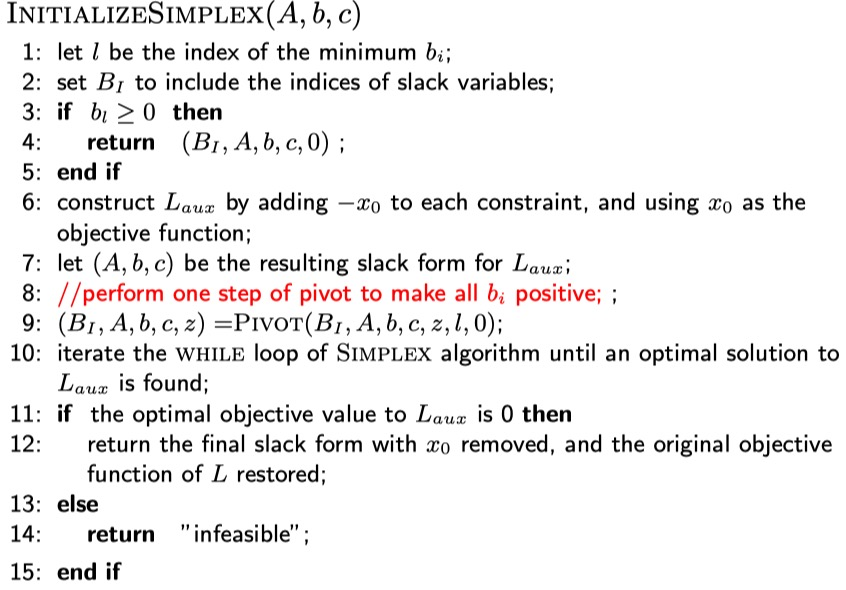
\includegraphics[scale=.5]{./1.png}
			\caption{Linear-inequality feasibility}
		\end{figure}
	
	\newpage
	\section{Interval Scheduling Problem}
	\subsection{Problem Description}
		A teaching building has m classrooms in total, and n courses are trying to use them. Each course $ i (i = 1, 2, · · · , n) $ only uses one classroom during time interval $ [S_i , F_i ) (F_i > S_i > 0) $. Considering any two courses can not be carried on in a same classroom at any time, you have to select as many courses as possible and arrange them without any time collision. For simplicity, suppose $ 2n $ elements in the set $ {S_1 , F_1 , · · · , S_n , F_n } $ are all different.
	
	\subsection{Solution}
		由题意可知,所给的$ 2n $个时间都是不同的,所以我们可以有$ 2n $个时间点,又因为题目要求每个时间段都最多只能有m门课同时上课,我们可以转化为每个时间点最多只有m门课在上课。比如在时间区间$ [S_k,F_k] $中,假设有如下的时间点$ {S_k,S_i,S_j,F_i,F_j,F_k} $,若第$ k $门课在上课,又因为第$ k $门课的时间区间为$ [S_k,F_k) $,那么我们可以将第$ k $门课的这些时间点设为$ (1,1,1,1,1,0) $,其中1表示第$ k $门课目前正在上课,0表示不在上课。
		
		首先,我们定义一些参数:

			$ m $, the maximum number of courses
			
			$ c_i,i\in[1,n] $
			
			$ x_{ij},i\in[1,n],j\in[1,2n] $

		\begin{equation*}
			c_i = \left\{
			\begin{array}{rlc}
			1, &if\ course\ i\ is\ choosed  \\
			0, &otherwise 
			\end{array}
			\right.
		\end{equation*}
		\begin{equation*}
			x_{ij} =\left\{
				\begin{array}{rlc}
					1, &course\ i\ occupy\ time\ point\ j\\
					0, &course\ i\ don't\ occupy\ time\ point\ j 
				\end{array}
			\right. 
		\end{equation*}
		
		
		因此问题可表达为:
			\begin{equation*}
				\begin{array}{rlc}
					max\ \ \    \sum_{i=1}^{n}c_i\ & \\
					s.t\ \ \   \sum_{i=1}^{n}x_{ij} &\le m ,for\ all\ j=1,2,\dots,2n\\
					      c_{i},x_{ij} &\in \{0,1\} , i\in[1,n],j\in[1,2n] 
				\end{array}
			\end{equation*}
			
		上面的公式也是标准型,不需要转换
		
	\subsection{Demo}
		设共有10门课,2个教室,每门课的时间如下所示:时间范围是[8,20],总计20个时间节点。
	
	各课程的时间如下:
		(( 14.5  18.5)
(  8.5  11. )
( 15.5  16.5)
( 11.5  18. )
( 10.5  15. )
( 12.5  16. )
( 10.   14. )
( 12.   19. )
( 13.   13.5)
(  9.   19.5))
		
		时间节点排序如下:
		
	8.5   9.   10.   10.5  11.   11.5  12.   12.5  13.   13.5  14.   14.5	15.   15.5  16.   16.5  18.   18.5  19.   19.5

	计算出每个课程占用的时间点如下所示:维度大小为$ 2n*n $:
	
	   0  1  2  3  4  5  6  7  8  9 10
	   
	 1  0  1  0  0  0  0  0  0  0  0
	 
	 2  0  1  0  0  0  0  0  0  0  1
	 
	 3  0  1  0  0  0  0  1  0  0  1
	 
	 4  0  1  0  0  1  0  1  0  0  1
	 
	 5  0  0  0  0  1  0  1  0  0  1
	 
	 6  0  0  0  1  1  0  1  0  0  1
	 
	 7  0  0  0  1  1  0  1  1  0  1
	 
	 8  0  0  0  1  1  1  1  1  0  1
	 
	 9  0  0  0  1  1  1  1  1  1  1
	 
	 10  0  0  0  1  1  1  1  1  0  1
	 
	 11  0  0  0  1  1  1  0  1  0  1
	 
	 12  1  0  0  1  1  1  0  1  0  1
	 
	 13  1  0  0  1  0  1  0  1  0  1
	 
	 14  1  0  1  1  0  1  0  1  0  1
	 
	 15  1  0  1  1  0  0  0  1  0  1
	 
	 16  1  0  0  1  0  0  0  1  0  1
	 
	 17  1  0  0  0  0  0  0  1  0  1
	 
	 18  0  0  0  0  0  0  0  1  0  1
	 
	 19  0  0  0  0  0  0  0  0  0  1
	 
	 20  0  0  0  0  0  0  0  0  0  0
	
		
		代码间附录A,运行结果如下,可见课程1、2、3、7、9被选中:
		
		\begin{figure}[htb]
			\centering
			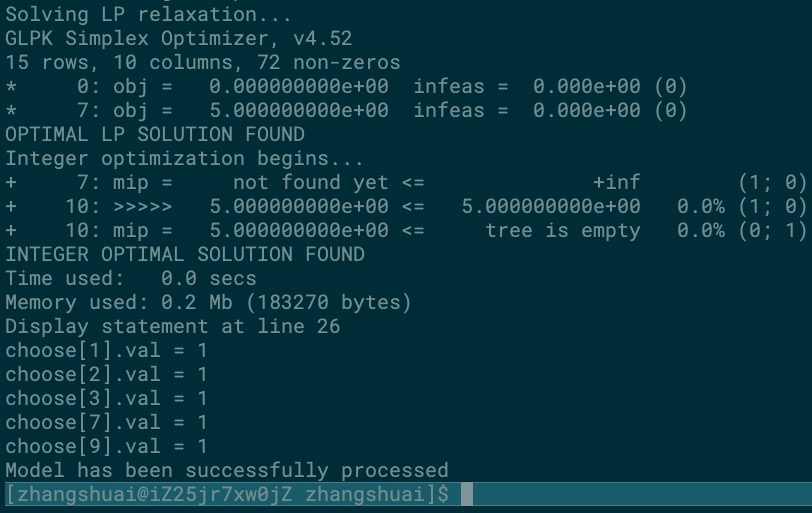
\includegraphics[scale=.7]{./schres.png}
			\caption{Interval Scheduling Problem}
		\end{figure}


	
	\newpage
	\newpage
	\section{Gas Station Placement}
	\subsection{Problem Description}
	
		Let’s consider a long, quiet country road with towns scattered very sparsely along it. Sinopec, largest oil refiner in China, wants to place gas stations along the road. Each gas station is assigned to a nearby town, and the distance between any two gas stations being as small as possible. Suppose there are n towns with distances from one endpoint of the road being $d_1 , d_2 , · · · , d_n$ . $ n $ gas stations are to be placed along the road, one station for one town. Besides, each station is at most $ r $ far away from its correspond town. $d_1 , d_2 , · · · , d_n$ and $ r $ have been given and satisfied $d_1 , d_2 , · · · , d_n,\ 0<r<d_1 $ and $ d_i + r < d_{i+1} − r $ for all $ i $. The objective is to find the optimal placement such that the maximal distance between two successive gas stations is minimized.
	
		Please formulate this problem as an LP.
	
	\subsection{Solution}
	
		由题意知,每个村镇都需要放置一个气站才能满足条件。
		
		首先定义参数:
		$ m $,要求的最大最小距离
		
		$ s_{i} $,表示第i个村镇放置的气站的位置
		
		$ d_i $,表示第i个村镇的位置
		
		$ r $,表示气站距离村镇的最大位置
		
		
		然后可以将问题表述成如下形式:
		\begin{align*}
		min\ \ \ \ \ \ \  \ \ \ \  \ \ \ \  & m\\ 
		s.t\ \ \ \ \ \ \  s_{i+1} - s_{i} &\le m&for\ all\ i=1,2,\dots,n-1 \\
		d_i - r &\le s_i \le d_i+r &for\ all\ i=1,2,\dots,n \\
		s_{i},m &\ge 0 &for\ all\ i=1,2,\dots,n
		\end{align*}
		
		转换为标准型:
		\begin{align*}
		min\ \ \ \ \ \ \  \ \ \ \  \ \ \ \  & m\\ 
		s.t\ \ \ \ \ \ \  s_{i+1} - s_{i} &\le m&for\ all\ i=1,2,\dots,n-1 \\
		-s_i &\le r - d_i  &for\ all\ i=1,2,\dots,n \\
		s_i &\le d_i+r &for\ all\ i=1,2,\dots,n \\
		s_{i},m &\ge 0 &for\ all\ i=1,2,\dots,n
		\end{align*}
		
	\subsection{Demo}
		设有10个村镇,它们与原点的距离为:[1] 10.0 [2] 25.89 [3] 39.48 [4] 58.42 [5] 69.72 [6] 82.82 [7] 99.6 [8] 116.77 [9] 128.52 [10] 147.85。
		
		参数r设为5.0
		
		代码在附录B,结果如下所示,可见,气站间的最大距离为14.21,气站的具体位置如图所示:
		
		\begin{figure}[htb]
			\centering
			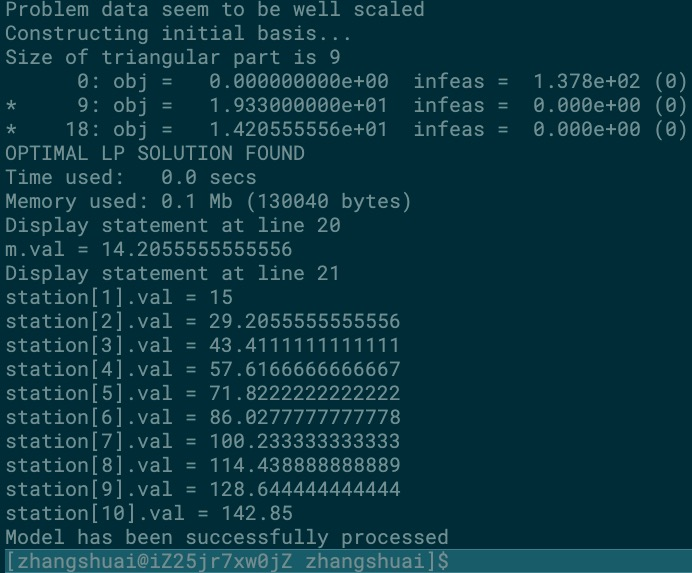
\includegraphics[scale=.7]{./gasres.png}
			\caption{Gas Station Placement}
		\end{figure}


	\end{CJK}	

\end{document} 
